\section{Introduction}
\label{sec:intro}
%
\begin{figure}[t!]
\centering
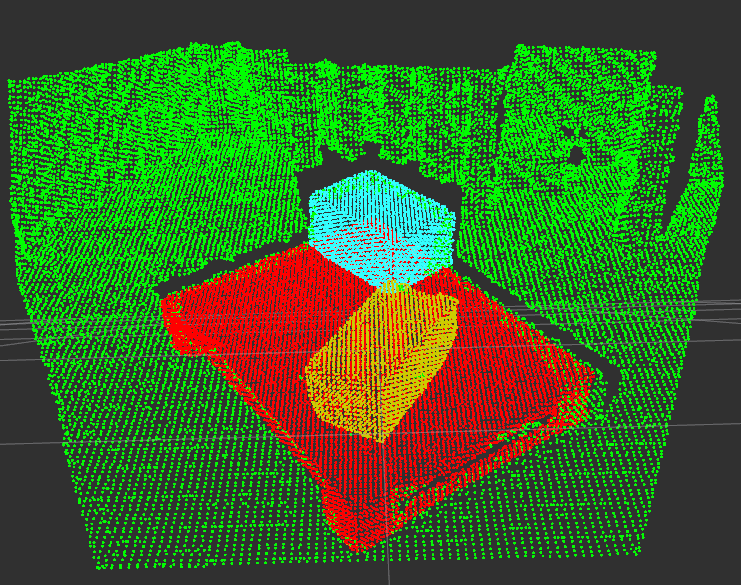
\includegraphics[width = \linewidth]{figs/setup}
\caption{The grasp envelope extraction procedure proposed in this work was used in an autonomous picking system, composed of the underactuated Velvet Fingers gripper~\cite{Tinc12} mounted on a KUKA LWR4+ robot arm (background). Experiments were performed to evaluate grasp acquisition success rates for the five test objects in the foreground. }
\label{fig:setup}
\end{figure}

Despite significant advances in gripper hardware design and in robot planning and control algorithms, autonomous grasp acquisition under uncontrolled conditions remains a challenging research problem.
On one hand, this is due to the necessity to solve a high-dimensional grasp- and motion planning problem for the full gripper-manipulator chain.
%
\par
%
The classical approach to reduce this complexity is to decouple the grasp synthesis problem by planning separately for the gripper and the manipulator.
To this end, state of the art grasping systems~\cite{Bere07,Srin10, Krug14a, Stoy15} often rely on sets of pre-computed grasps. 
At runtime, these grasps are evaluated by a motion planner and executed in an open-loop fashion, or in combination with perceptual feedback ($e.\,g.$, visual servoing).
